\newpage
\subsection{GPIO/UART/I2C/1-Wire interfaces}

\begin{figure}[ht]
  \begin{center}
    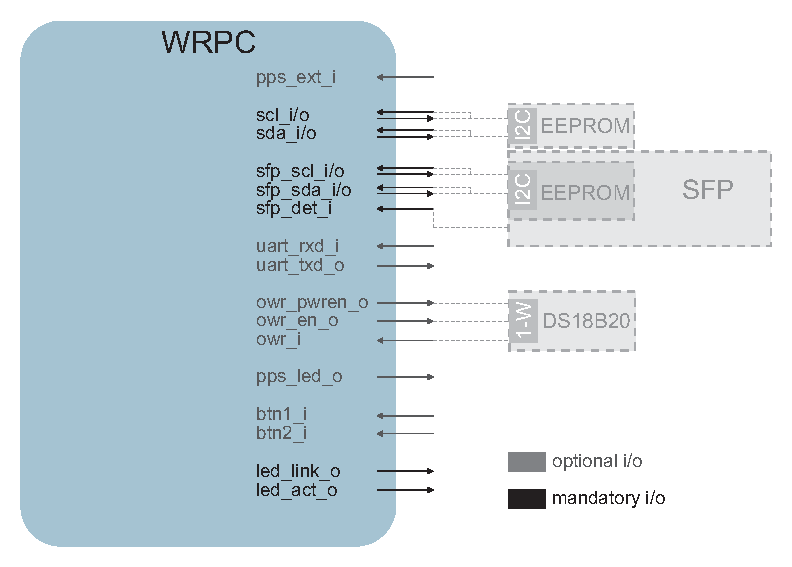
\includegraphics[width=.9\textwidth]{fig/basic_wrpc_gpio.pdf}
    \caption{Other interfaces of WRPC}
  \end{center}
\end{figure}

Other hardware peripherals can be connected to the White Rabbit PTP
Core. It has a UART, 1-Wire and two $I^2C$ interfaces implemented
inside. The $I^2C$ connection to the SFP module
is used to read its Part ID, while the external EEPROM stores calibration
values for each supported SFP together with an initialization script. That script
is executed every time the WRPC is powered on and can contain instructions to
automatically match the SFP's Part ID with the EEPROM content and load appropriate
calibration values. The SFP presence indicator is mandatory and has to be connected.
Otherwise, the WRPC won't be able to operate properly (without knowing whether
the SFP transceiver is actually inserted).

Furthermore, a 1-Wire digital thermometer provides
on-board temperature, but also its unique ID is used to calculate default MAC
address of the physical Ethernet interface. The UART interface provides a user shell
that can be used to interact with the White Rabbit PTP Core. More detailed
description of the WRPC shell can be found in the \emph{White Rabbit PTP Core User's
Manual - Building and Running} \cite{wrpc_man}.

\begin{center}
  \begin{tabular}{|p{3cm}|l|p{11cm}|}
    \hline
    {\bf Signal name} & {\bf size} & {\bf description} \\
    \hline \hline
    \texttt{pps\_ext\_i} & 1 & [optional] external 1-PPS input used in
    GrandMaster mode\\
    \hline
    \texttt{scl\_i} \linebreak \texttt{scl\_o} \linebreak \texttt{sda\_i} \linebreak
    \texttt{sda\_o} & 4 & I2C interface for EEPROM memory storing calibration
    parameters and WRPC init script\\
    \hline
    \texttt{sfp\_scl\_i} \linebreak \texttt{sfp\_scl\_o} \linebreak
    \texttt{sfp\_sda\_i} \linebreak \texttt{sfp\_sda\_o} & 4 & I2C interface for
    EEPROM inside SFP module\\
    \hline
    \texttt{sfp\_det\_i} & 1 & SFP presence indicator\\
    \hline
    \texttt{uart\_rxd\_i} \linebreak \texttt{uart\_txd\_o} & 2 & [optional] serial
    UART interface for interaction with WRPC software\\
    \hline
    \texttt{owr\_pwren\_o} \linebreak \texttt{owr\_en\_o} \linebreak \texttt{owr\_i} &
    3 & [optional] 1-Wire interface used to read the temperature of hardware board from
    digital thermometer (e.g. Dallas DS18B20)\\
    \hline
    \texttt{pps\_led\_o} & 1 & 1-PPS signal with extended pulse width to drive a
    LED\\
    \hline
    \texttt{btn1\_i} \linebreak \texttt{btn2\_i} & 2 & two microswitch inputs,
    active low, currently not used in official WRPC software\\
    \hline
    \texttt{led\_link\_o} & 1 & signal for driving Ethernet Link LED\\
    \hline
    \texttt{led\_act\_o} & 1 & signal for driving Ethernet Act LED\\
    \hline
  \end{tabular}
\end{center}
